

\tikzset{every picture/.style={line width=0.75pt}} %set default line width to 0.75pt        

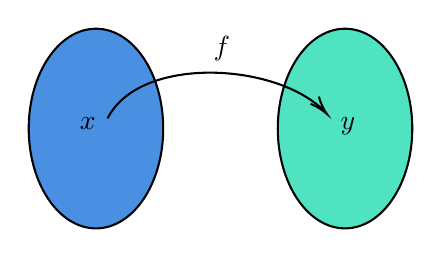
\begin{tikzpicture}[x=0.75pt,y=0.75pt,yscale=-1,xscale=1, scale = 0.8]
%uncomment if require: \path (0,300); %set diagram left start at 0, and has height of 300

%Flowchart: Connector [id:dp590735645517438] 
\draw  [fill={rgb, 255:red, 74; green, 144; blue, 226 }  ,fill opacity=1 ] (50,90.13) .. controls (50,56.92) and (68.13,30) .. (90.5,30) .. controls (112.87,30) and (131,56.92) .. (131,90.13) .. controls (131,123.33) and (112.87,150.25) .. (90.5,150.25) .. controls (68.13,150.25) and (50,123.33) .. (50,90.13) -- cycle ;
%Flowchart: Connector [id:dp9948606826522155] 
\draw  [fill={rgb, 255:red, 80; green, 227; blue, 194 }  ,fill opacity=1 ] (200,90.13) .. controls (200,56.92) and (218.13,30) .. (240.5,30) .. controls (262.87,30) and (281,56.92) .. (281,90.13) .. controls (281,123.33) and (262.87,150.25) .. (240.5,150.25) .. controls (218.13,150.25) and (200,123.33) .. (200,90.13) -- cycle ;
%Curve Lines [id:da3293081752285161] 
\draw    (97.5,84) .. controls (116.71,45.83) and (199.46,50.11) .. (228.22,79.87) ;
\draw [shift={(229.5,81.25)}, rotate = 228.42] [color={rgb, 255:red, 0; green, 0; blue, 0 }  ][line width=0.75]    (10.93,-3.29) .. controls (6.95,-1.4) and (3.31,-0.3) .. (0,0) .. controls (3.31,0.3) and (6.95,1.4) .. (10.93,3.29)   ;

% Text Node
\draw (79,81.9) node [anchor=north west][inner sep=0.75pt]    {$x$};
% Text Node
\draw (236,81.4) node [anchor=north west][inner sep=0.75pt]  [color={rgb, 255:red, 0; green, 0; blue, 0 }  ,opacity=1 ]  {$y$};
% Text Node
\draw (159.5,32.4) node [anchor=north west][inner sep=0.75pt]    {$f$};


\end{tikzpicture}
